\begin{figure}[!ht]
\centering
    \begin{subfigure}{0.43\linewidth}
        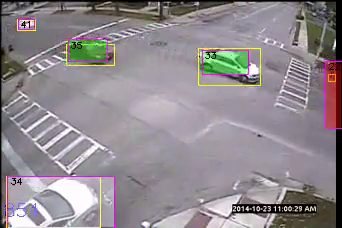
\includegraphics[width=\linewidth]{./img/gp/193402-kf-1.png}
        \subcaption{Kalman filter with Linear model.}
        \label{subfig:kf-1}
    \end{subfigure}
    \begin{subfigure}{0.43\linewidth}
        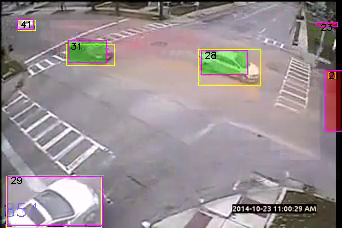
\includegraphics[width=\linewidth]{./img/gp/193402-gp-1.png}
        \subcaption{Kalman filter with non-linear model.}
        \label{subfig:gp-1}
    \end{subfigure}%
    \caption{Tracking screenshots at frame 854, no trajectory for Gaussian Process.}
    \label{fig:kf-gp-1}
\end{figure}

\begin{figure}
\centering
    \begin{subfigure}{0.43\linewidth}
        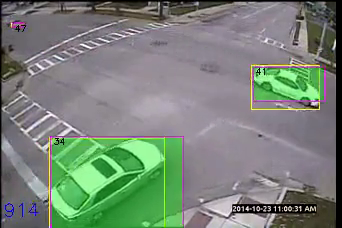
\includegraphics[width=\linewidth]{./img/gp/193402-kf-2.png}
        \subcaption{Kalman filter with linear model.}
        \label{subfig:kf-2}
    \end{subfigure}
    \begin{subfigure}{0.43\linewidth}
        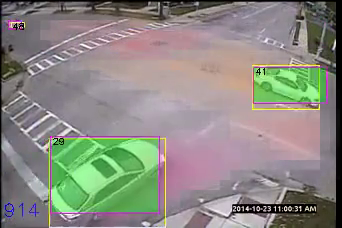
\includegraphics[width=\linewidth]{./img/gp/193402-gp-2.png}
        \subcaption{Kalman filter with non-linear model.}
        \label{subfig:gp-2}
    \end{subfigure}%
    \caption{Tracking screenshots at frame 914, 1-2 trajectories for Gaussian Process.}
    \label{fig:kf-gp-2}
\end{figure}

\begin{figure}
\centering
    \begin{subfigure}{0.43\linewidth}
        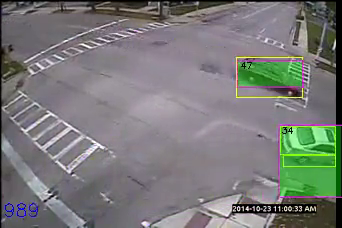
\includegraphics[width=\linewidth]{./img/gp/193402-kf-3.png}
        \subcaption{Kalman filter with linear model.}
        \label{subfig:kf-3}
    \end{subfigure}
    \begin{subfigure}{0.43\linewidth}
        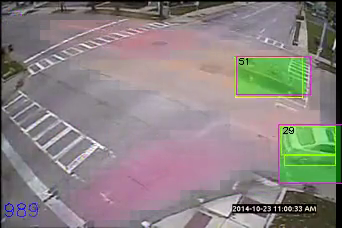
\includegraphics[width=\linewidth]{./img/gp/193402-gp-3.png}
        \subcaption{Kalman filter with non-linear model.}
        \label{subfig:gp-3}
    \end{subfigure}%
    \caption{Tracking screenshots at frame 989, 5-8 trajectories for Gaussian Process.}
    \label{fig:kf-gp-3}
\end{figure}